
In Chapter \ref{subsec:controltool} ....



\begin{figure}[h]
	\centering
	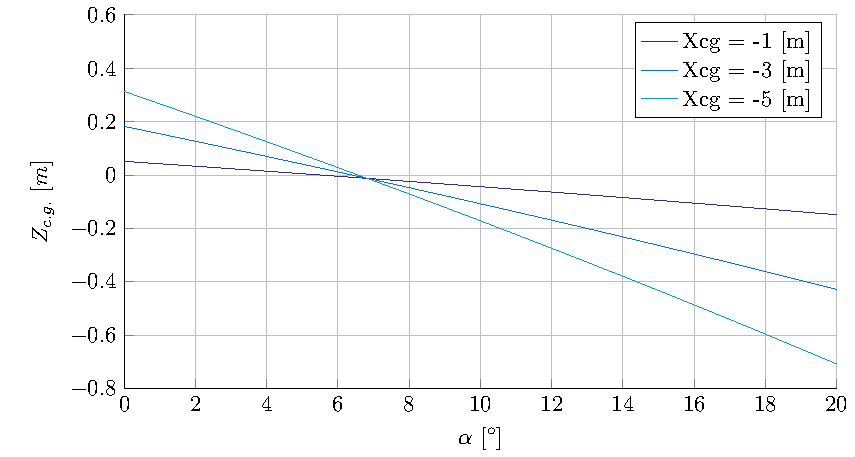
\includegraphics[width=0.8\textwidth]{./Figure/control/moment}
	\caption{1}
	\label{fig:}
\end{figure}


\paragraph{Control system selection}



\paragraph{Control system results}

The results of the control system can be subdivided into two components. The control system mass and its corresponding accuracy.

Mass estimates are based on the required propellant mass, thruster mass and fuel tank mass. The propellant mass can be subdivided into a further two categories: the control within the atmosphere and the control outside of the atmosphere. General equation were previously discussed within section \ref{subsec:controltool}.

\subparagraph{Control within the atmosphere} 

Within the Martian atmosphere control is performed on the basis of banking. A control system featuring a single bank control reversal is always able to derive at the destination with a average accuracy of 1.009 [$km$]\cite{Lu2007} at Mars. The control system accuracy can further be significantly reduced by using multiple bank reversals, reducing mainly the dispersions observed. 

Accuracies where obtained using dispersions with a \gls{sym:CL} of $\pm 0.03 $, \gls{sym:CD}  of $\pm 0.06 $ and mass and atmospheric dispersion of 5\% and 30\% respectively \cite{Lu2007}. Accuracies up of 10[$m$] are achieved if the staging and final descent are included \cite{Davis2010}. 

It is argued that with an increasing amount of bank reversals, complemented with additional control measures higher accuracies can be obtained. The trajectories are budgeted for a total of six bank reversals for both the initial aero-capture and the final \gls{edl}. Six bank reversals are typical values for single orbit \cite{Lu2007, Cianciolo2010}. A very qualitative definition of six bank reversels as defined within the control system analysis is displayed in Figure \ref{fig:bankdef}

\begin{figure}[h]
	\centering
	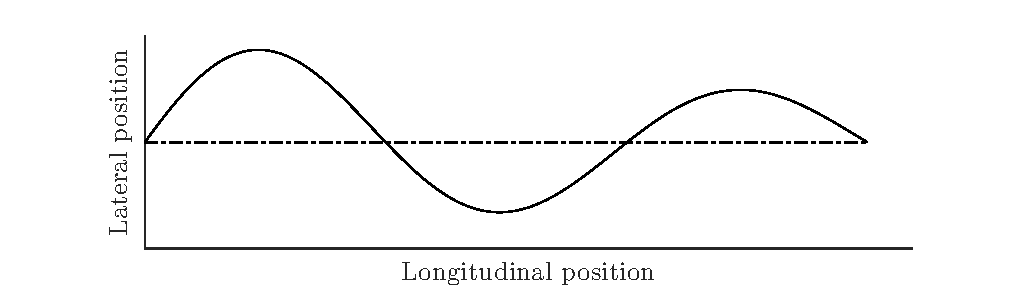
\includegraphics[width=0.8\textwidth]{./Figure/control/bankdef.eps}
	\caption{Qualitative figure displaying six bank reversals}
	\label{fig:bankdef}
\end{figure}


The mass estimates are moreover based on peak rotational rates of 20 [$deg\cdot s^{-1}$] and 5 [$deg \cdot s^{-2}$] as used by Davis et al. \cite{Davis2010}.

The inertial moments are based on a homogeneous mass distribution and a simplified geometric shape. The crew module is assumed to be a hollow cylinder with the structural components attached to the in and outside of this cylinder. The inflatable structure is assumed to be of a circular disk shape, again with a homogeneous mass distribution. Within this shape the mass is assumed to be primarily situated on the outside of the spacecraft such that conservative mass estimates will be achieved.


\subparagraph{Control outside the atmosphere}

Control outside the Martian atmosphere 


\subparagraph{Thruster}

Inertial moments combined with rotational rates deliver the required control moments via Equation \ref{eq:mcontrol}. For the most efficient performance the thruster are placed on the outside of the Centerbody. Although thrusters placed on the outside of the inflatable are able to generate higher torques, multiple disadvantages hinder this placement:

\begin{itemize}
\item Thruster place on the inflatable will difficult the deployment
\item Deformation of the inflatable, and thus the thrusters performance is difficult to predict.
\item Placement of thrusters on the inflatable may induce disadvantageous vibrations or aeroelastic effects.  
\end{itemize} 

Thruster performance requirements are primarily based on the bank control speed. Apocenter velocity increments are assumed to be performed by the pre-existing thruster which are used for the boost to the transfer orbit. The thruster used for creating the bank control moments require a peak thrust of around 900 [$N$]. Torque is provided by multiple thrusters such that partial operations may continue if a single thrusters fails.
 Indicative values are for a capable thruster are for example given by the  MONARC-445 hydrazine thruster\footnote{URL: \url{http://www.moog.com/literature/Space\_Defense/Spacecraft/Propulsion/Monopropellant\_Thrusters\_Rev\_0613.pdf} Accessed 15 June 2015}. The MONARC-445 thruster delivers a nominal thrust of 445[$N$] at a weight of 1.6[$kg$].  A eightfold of these thrusters allows for control around the roll axis and moreover provides partial control in the case of failure of one such thruster.
 
 
Specific preference lies in the use of hydrazine as propellant such that it is interchangeable with the remaining propellent requiring systems. The use of a single propellant allows for lower fuel fractions as propellants margins required for the different mission phases can be combined.

Additionally thrusters for the velocity increments in the apocenter are required. These are considered in the mass estimate of the crewmodule as these can already be used for the more intensive injection from \gls{leo} to the transfer orbit. Again hydrazine thrusters are considered for interchangeability throughout the various mission stages. This is however combined with a second propellent as for bi-propellant thrusters as this yields significant performance increase (in terms of \gls{sym:Isp})\cite{Wertz2011}. 

A thruster suitable for such a purpose is the unified propulsion system by Japan IHI at a weight of 15.7 [$kg$] and a specific impulse of 321.4 [$s$]. As secondary propellant NTO is required.



